% CHAPITRE 2
% SUIVI VARIABILITE SPATIALE

\chapter{Sites d'études et méthodologies employées}
\newpage

\section{Présentation du site d'étude}

\begin{figure}
\centering
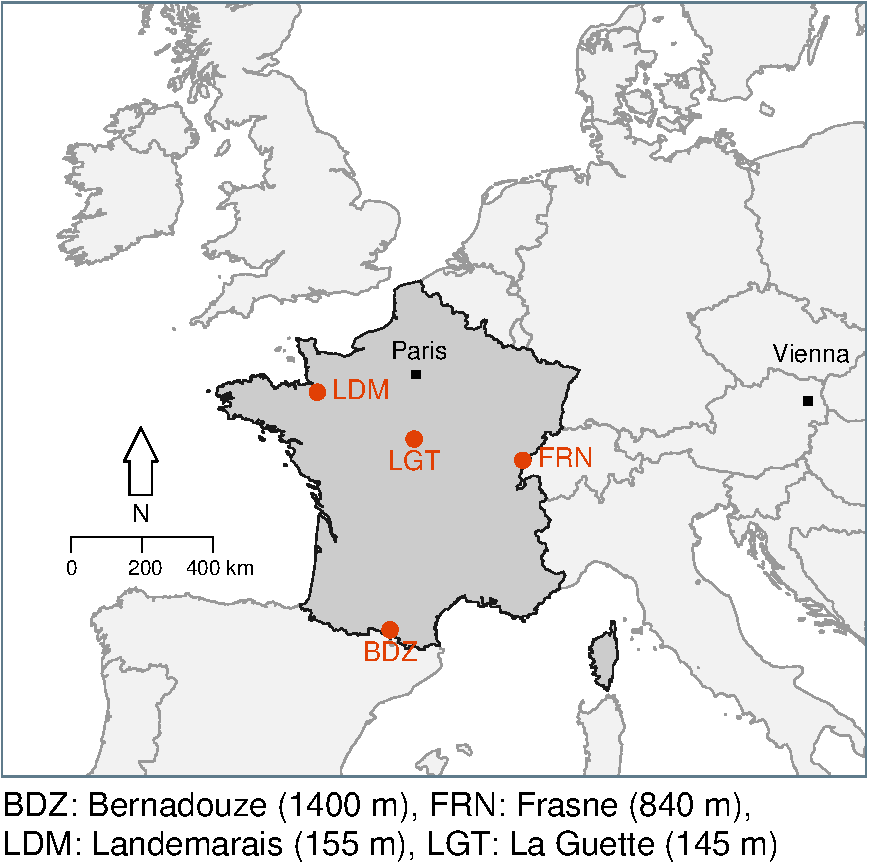
\includegraphics[width=.75\textwidth]{chap2/SNO_siteLocalisation}
\caption{Site d'études SNO}
\label{fig:tair}
\end{figure}


L'ensemble des sites d'études sont regroupés au sein d'un service d'observation

%\subsection{La Guette}

La tourbière de La Guette est situé à Neuvy-sur-Barangeon, en Sologne, dans le département du Cher.
Le site s'étend sur une surface d'une vingtaine d'hectare avec une géométrie relativement allongée.
Avec une conductivité généralement inférieur à 80 uS/m2 et un pH compris entre 4 et 5 elle se classe parmis les "transitionnal poor fen"
Les datations effectuées sur le site permettent de dire que la tourbière est agée de 5 à 6000 ans.
Dans les années 19XX la construction d'une route coupe la tourbière dans sa partie sud.
En 2008 le récurage du fossé de drainage bordant la route semble entrainer une augmentation significative des pertes d'eau du système.

Des travaux (SOURCE, Émelie) d'analyse de photos aériennes ont ainsi montré une progression importante du boisement (principalement des pins (pinus Sylvestris) et des bouleau (Betula sp.). Des herbacées envahissent également le site avec une forte présence de la molinie (Molinia caerulea)

Sont présente sur le site un certain nombre d'espèces caractéristiques des tourbières comme les sphaignes (principalement Sphagnum cuspidatum et Sphagnum rubellum) et Eriophorum augustifolium.

\begin{figure}
\centering
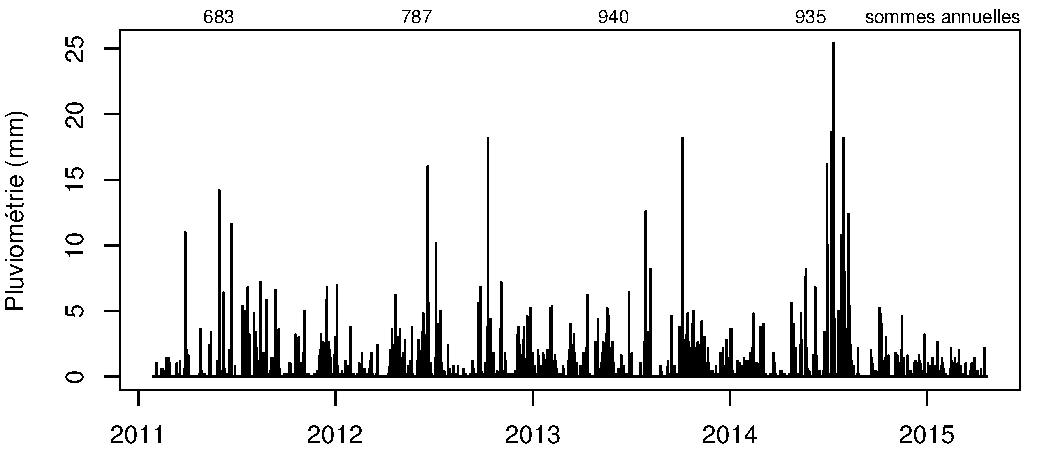
\includegraphics[width=\textwidth]{chap2/pluvio}
\caption{Évolution du niveau de la pluviométrie, en \si{\mm}, des années 2011 à 2014}
\label{fig:pluvio}
\end{figure}

\begin{figure}
\centering
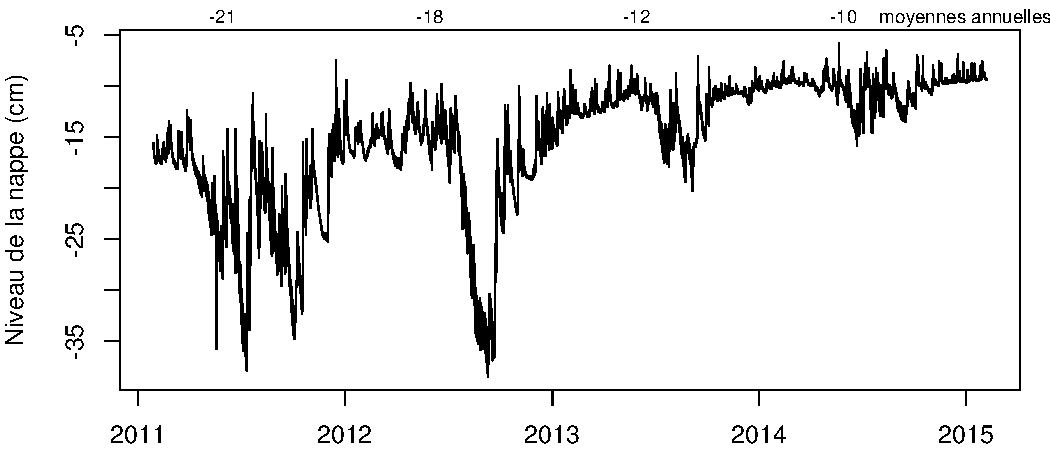
\includegraphics[width=\textwidth]{chap2/WTL}
\caption{Évolution du niveau de la nappe, en cm par rapport à la surface, des années 2011 à 2014}
\label{fig:WTL}
\end{figure}

Au cours des dernières années, les précipitations sont relativement différentes avec deux années plus sèche que la moyenne avant 2013 et deux années plus humide en 2013 et 2014 (Figure~\ref{fig:pluvio}).
On observe également cette dualité au niveau du niveau de la nappe.
Avant 2013 les étés sont marqués par des étiages important avec des baisses du niveau de nappe allant jusqu'à \SI{-60}{\cm} en 2012 (Figure~\ref{fig:WTL}).
Après 2013, les étiages sont beaucoup moins importants sur le site.



\begin{figure}
\centering
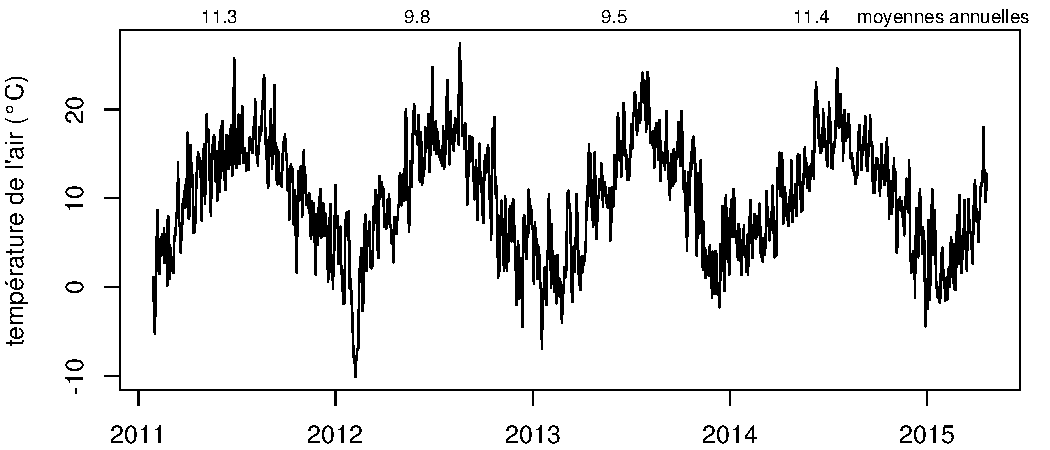
\includegraphics[width=\textwidth]{chap2/tair}
\caption{Évolution de la température de l'air (en \textdegree C) des années 2011 à 2014}
\label{fig:tair}
\end{figure}



Au sein de ses sites de nombreuses mesures ont été effectuée et notamment des mesures de flux de GES à la fois concernant le CO2 et le CH4. La méthodologie étant transverse à de nombreuses expérimentations il convient de l'expliquer au préalable.

\section{Mesures de flux}
\label{sec:clsd_chbr_method}

Il existe de nombreuses façon de mesurer des flux de gaz. 
Des méthodes globale comme les tour à flux utilisant des méthodes d'Eddy Covariance. 
Des méthodes plus locale, les chambres d'accumulation de gaz qui peuvent être statique ou dynamique, selon que la sonde mesurant le gaz soit directement dans la chambre ou que le gaz soit apportée à cette dernière via un système de pompe. Elles peuvent être ouverte ou fermée.

La méthode de mesure retenue pour ces travaux est l'utilisation de chambre statique fermée, permettant une mesure locale et directe des flux.
Pour cela des embases sont placées sur le terrain.
Ce sont des cylindres en PVC de \SI{31}{\centi\metre} de diamètre, et d'une hauteur de \SI{15}{\centi\metre} ont été installé dans la tourbière en les insérant de 8 à \SI{10}{\centi\metre}.
La partie basse de leurs parois, située sous la surface du sol après installation, est préalablement percée afin de minimiser les effets de l'embase sur l'écoulement de l'eau et le développement racinaire.
Les embases sont généralement posée 12h avant toute mesure afin de ne pas mesurer de dégagement gazeux liés à l'installation.

Que mesure-t-on ?
Le plus souvent 2 mesures consécutives sont effectuées la première avec une chambre transparente permettant d'accéder à la NEE et l'autre avec une chambre recouverte d'un isolant permettant de bloquer la lumière et permettant de mesurer les respirations. (pourquoi les respirations?)

De nombreux écueils peuvent rendre une mesure inexploitable. D'abord le placement de la chambre, cela peut sembler trivial mais positionner la chambre au milieu d'herbacées et de bruyère n'est pas tourjours évident. Plus anectdotiquement des sphaignes gelées, recouvrant les bords de l'embase rendent la pose de la chambre difficile voire impossible. Selon l'heure de la journée des gradients de concentrations peuvent être présent et augmenter localement les concentrations de CO2 de façon importante allant jusqu'à saturer la sonde.

Au vu du volume de données acquises et souhaitant garder l'intérêt de mesure manuelle, à savoir le contrôle humain des flux et des conditions de mesure, il a été nécessaire de développer un outil de traitement facilitant le contrôle et le calcul des flux.
Ceci afin d'éviter de recourir à des seuils arbitraires (typiquement une valeur de R$^{2}$) pour le contrôle qualité des données, mais également de permettre une reproductibilité et un traçage des modifications effectuées sur les données brutes.
(donner des exemples)

QUESTIONS :

*Taille des embases ? Effets de bord ?
*Perturbation du milieu ? (Mesure de végétation, pose de la chambre, mesure pièzo...)
*Impact de la strate arborée ?
*Validité des profils de température ?
Méthode de Chambre fermée (Biais ?)

Améliorations ? (Lister les amélioration à faire ou non)


\section{Facteurs contrôlants}
Afin de déterminer l'impact de facteurs contrôlants sur ces flux, mesurer les flux ne suffit pas il faut également mesurer les variables environnementales dont on pense qu'elles seront des facteurs contrôlants important.
La description des techniques et matériels communs aux différentes expérimentations utilisées est développée ci-dessous.
Par contre leur mise en œuvre ou caractéristiques spécifiques, comme la fréquence des mesures, sera décrite individuellement au niveau des parties détaillant chacune des expérimentations.

\subsection{acquisitions automatisées}

Les paramètres météorologiques ont été mesurés, en un point, au centre de la tourbière (\textbf{carte ?}) à l'aide d'une station d'acquisition Campbell installée sur le site en 2008.
Les variables ont été acquises à une fréquence horaire jusqu'au 20 février 2014 puis toutes les demi-heures par la suite. 
Les paramètres enregistrés sont la pression atmosphérique, l'humidité relative de l'air, la pluviométrie, l'irradiation solaire, la vitesse et la direction du vent. (\textbf{détail du matos ?}).
Cette même station à également permis l'acquisition de la température de l'air et de la tourbe à \num{-5}, \num{-10}, \num{-20} et \SIlist{-40}{\cm}.
Installées à la même époque, quatre sondes \textbf{OTT ?} de mesure du niveau de la nappe d'eau permettent le suivi du niveau de la nappe dans la tourbière.

\subsection{Protocole d'estimation de la végétation}

Le suivi non-destructif d'une végétation n'est pas triviale et nécessite la mise en place de protocoles particuliers en fonction du type de végétation.
L'objectif est de pouvoir estimer une biomasse produite en impactant au minimum la végétation en place.
Pour l'ensemble des espèces végétales présentes dans les embases servant à la mesure des flux un recouvrement à été estimé, à l’œil.


\subsubsection{La strate arbustive}
Pour la strate arbustive des mesures de hauteur moyenne ont été effectuées, en mesurant depuis le niveau du sol, ou le toit des sphaignes, si elles étaient présentes, jusqu'au sommet de l'individu.
\begin{figure}
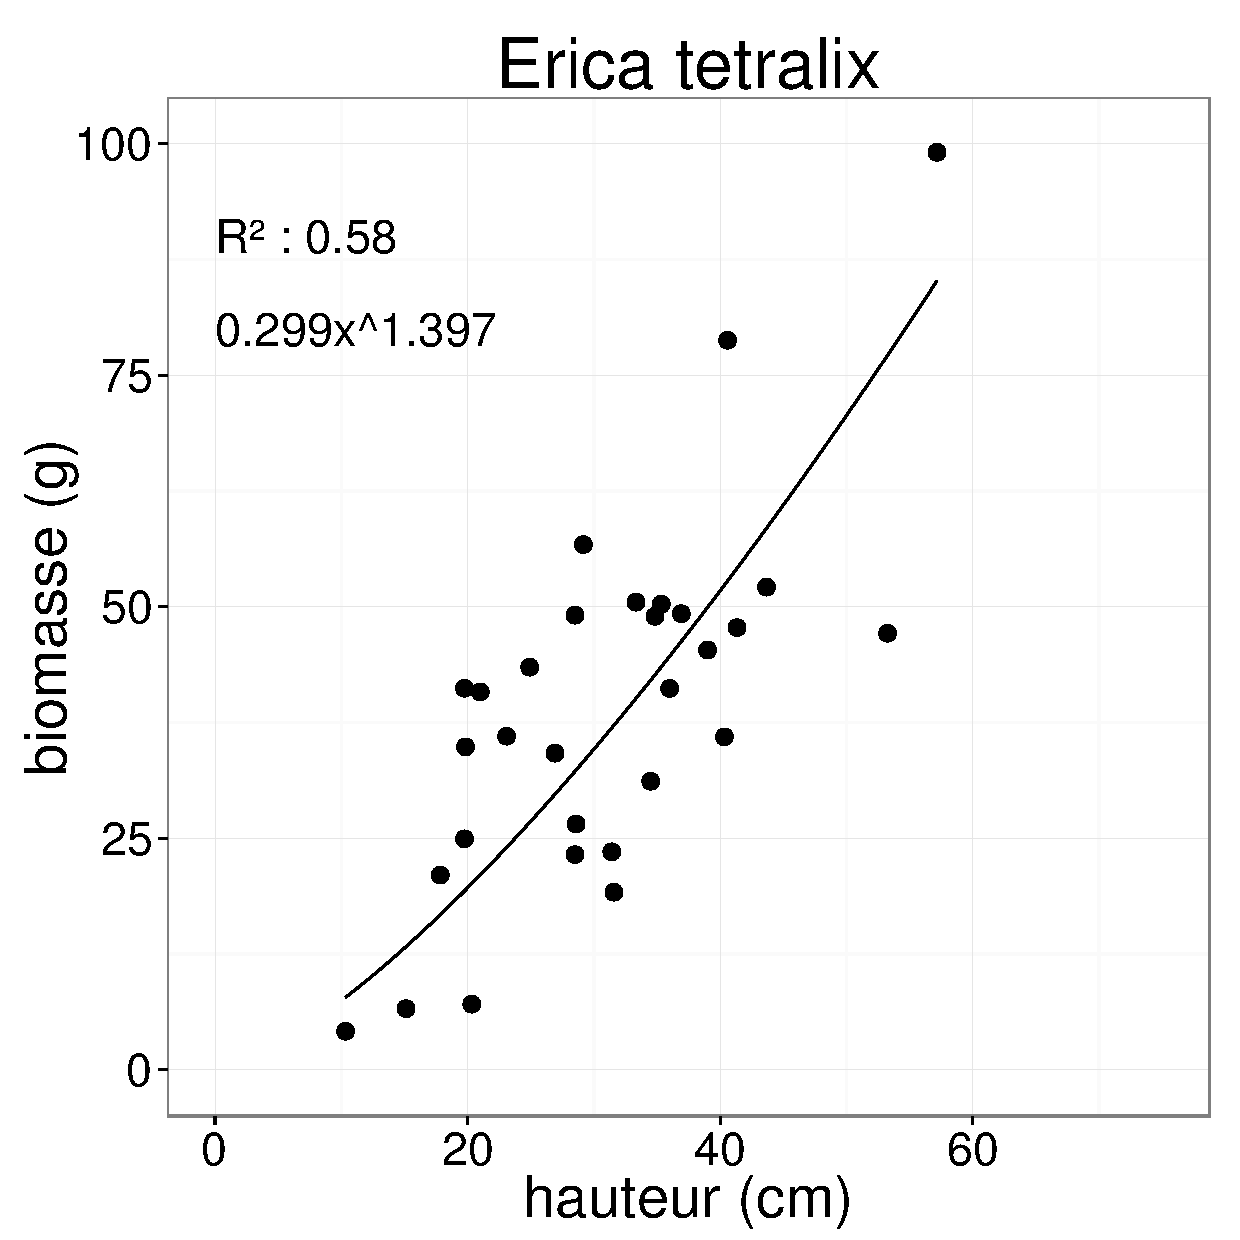
\includegraphics[width=.5\textwidth]{chap2/cal_tetra_eq}
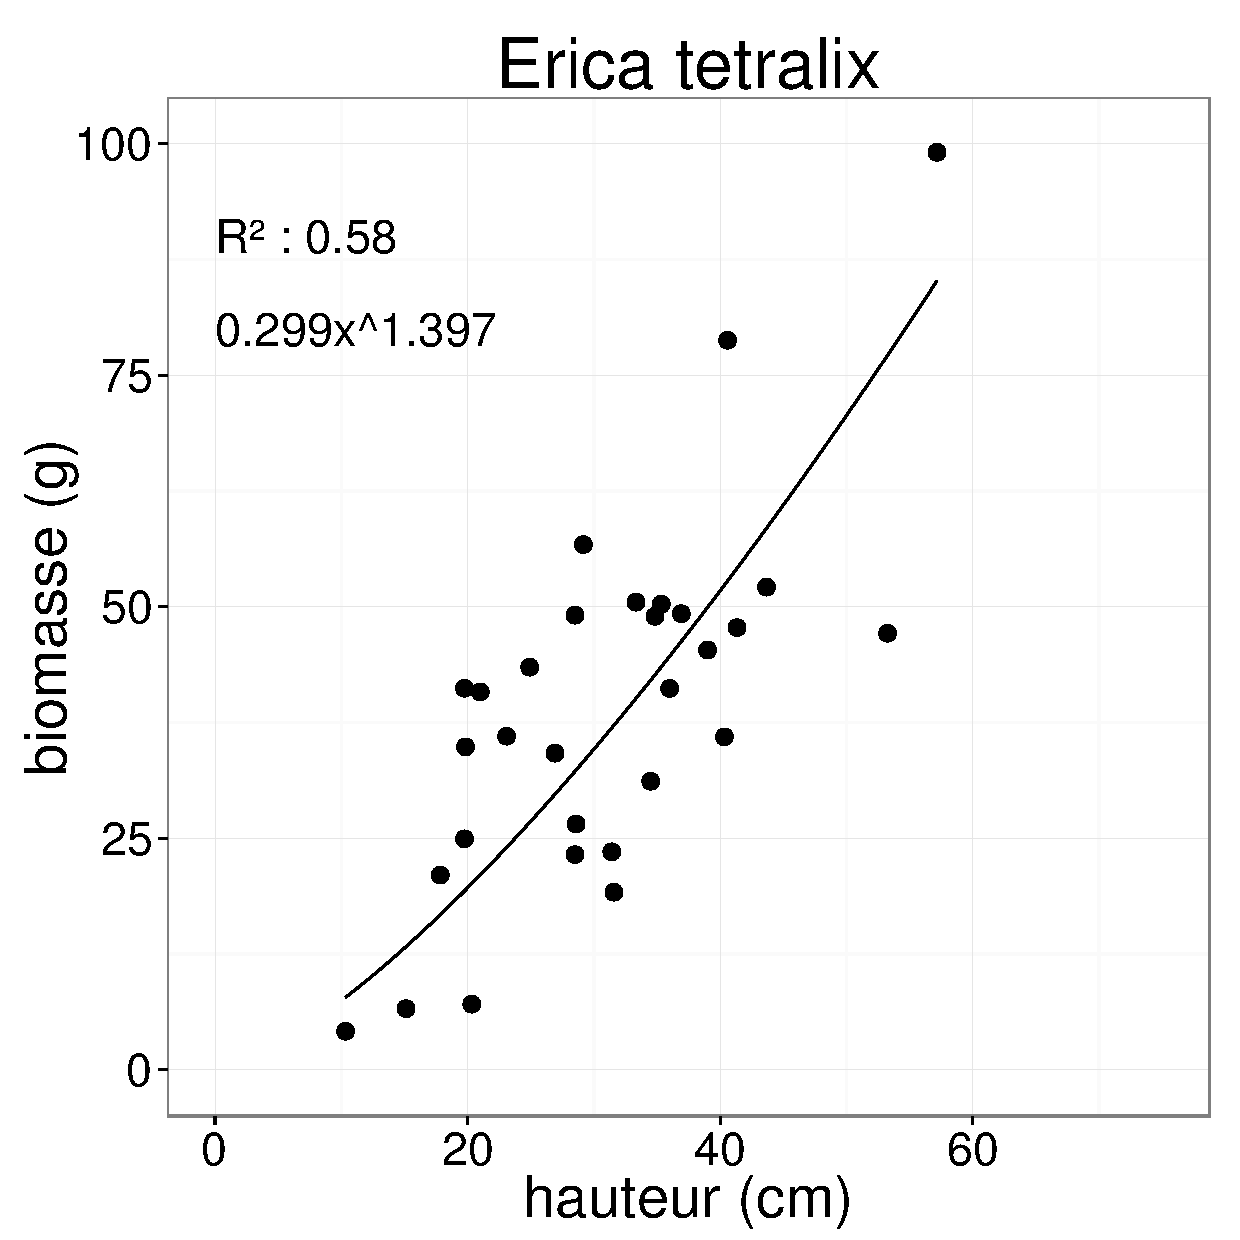
\includegraphics[width=.5\textwidth]{chap2/cal_tetra_eq}
\caption{Calibration de la biomasse en fonction de la hauteur}
\label{fig:cal_arbu}
\end{figure}

\subsubsection{La strate herbacée}
Pour la strate herbacée, en 2013, 5 individus des deux espèces majoritaires (Eriophorum vaginatum ? augustifolium ?, Molinia Caerulea) ont été marqués afin de pourvoir les mesurer plusieurs fois au cours de la saison.
Cependant les difficultés à retrouver les individus marqués couplés à la mort d'un nombre important d'entre eux n'ont pas permis d'acquérir de résultats significatifs.
En conséquence en 2014 ces deux espèces ont fait l'objet de comptage exhaustif et de mesure de hauteur moyenne.


\begin{figure}
	\centering
	\begin{subfigure}[t]{0.5\textwidth}
		\centering
		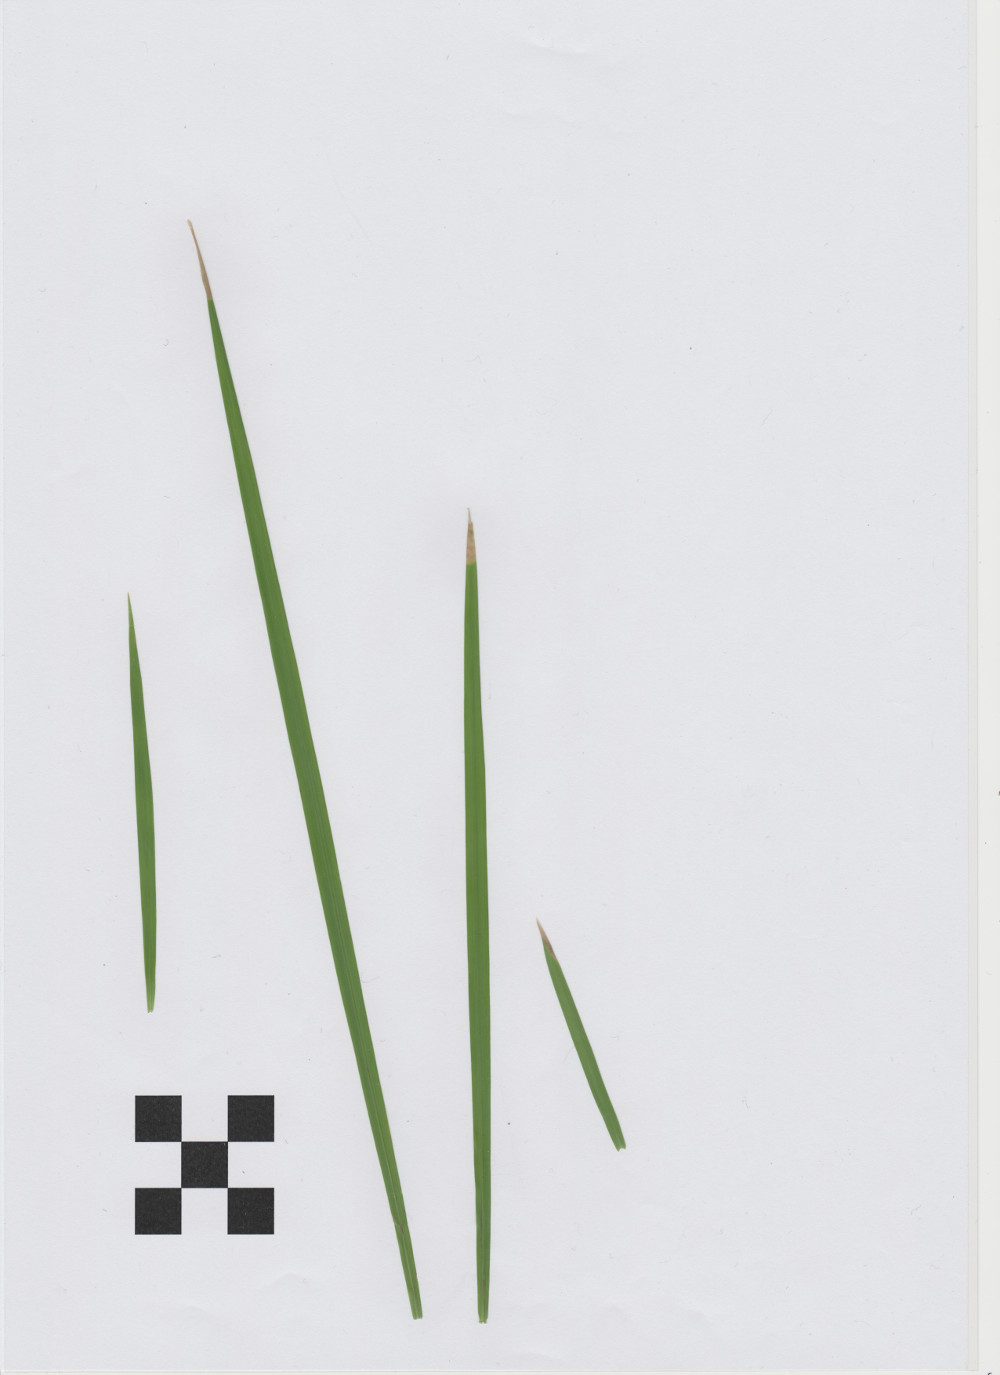
\includegraphics[width=.8\textwidth, frame]{chap2/Cch_moli_A_1to4}
		\caption{image scannée}
	\end{subfigure}%
	\begin{subfigure}[t]{0.5\textwidth}
		\centering
		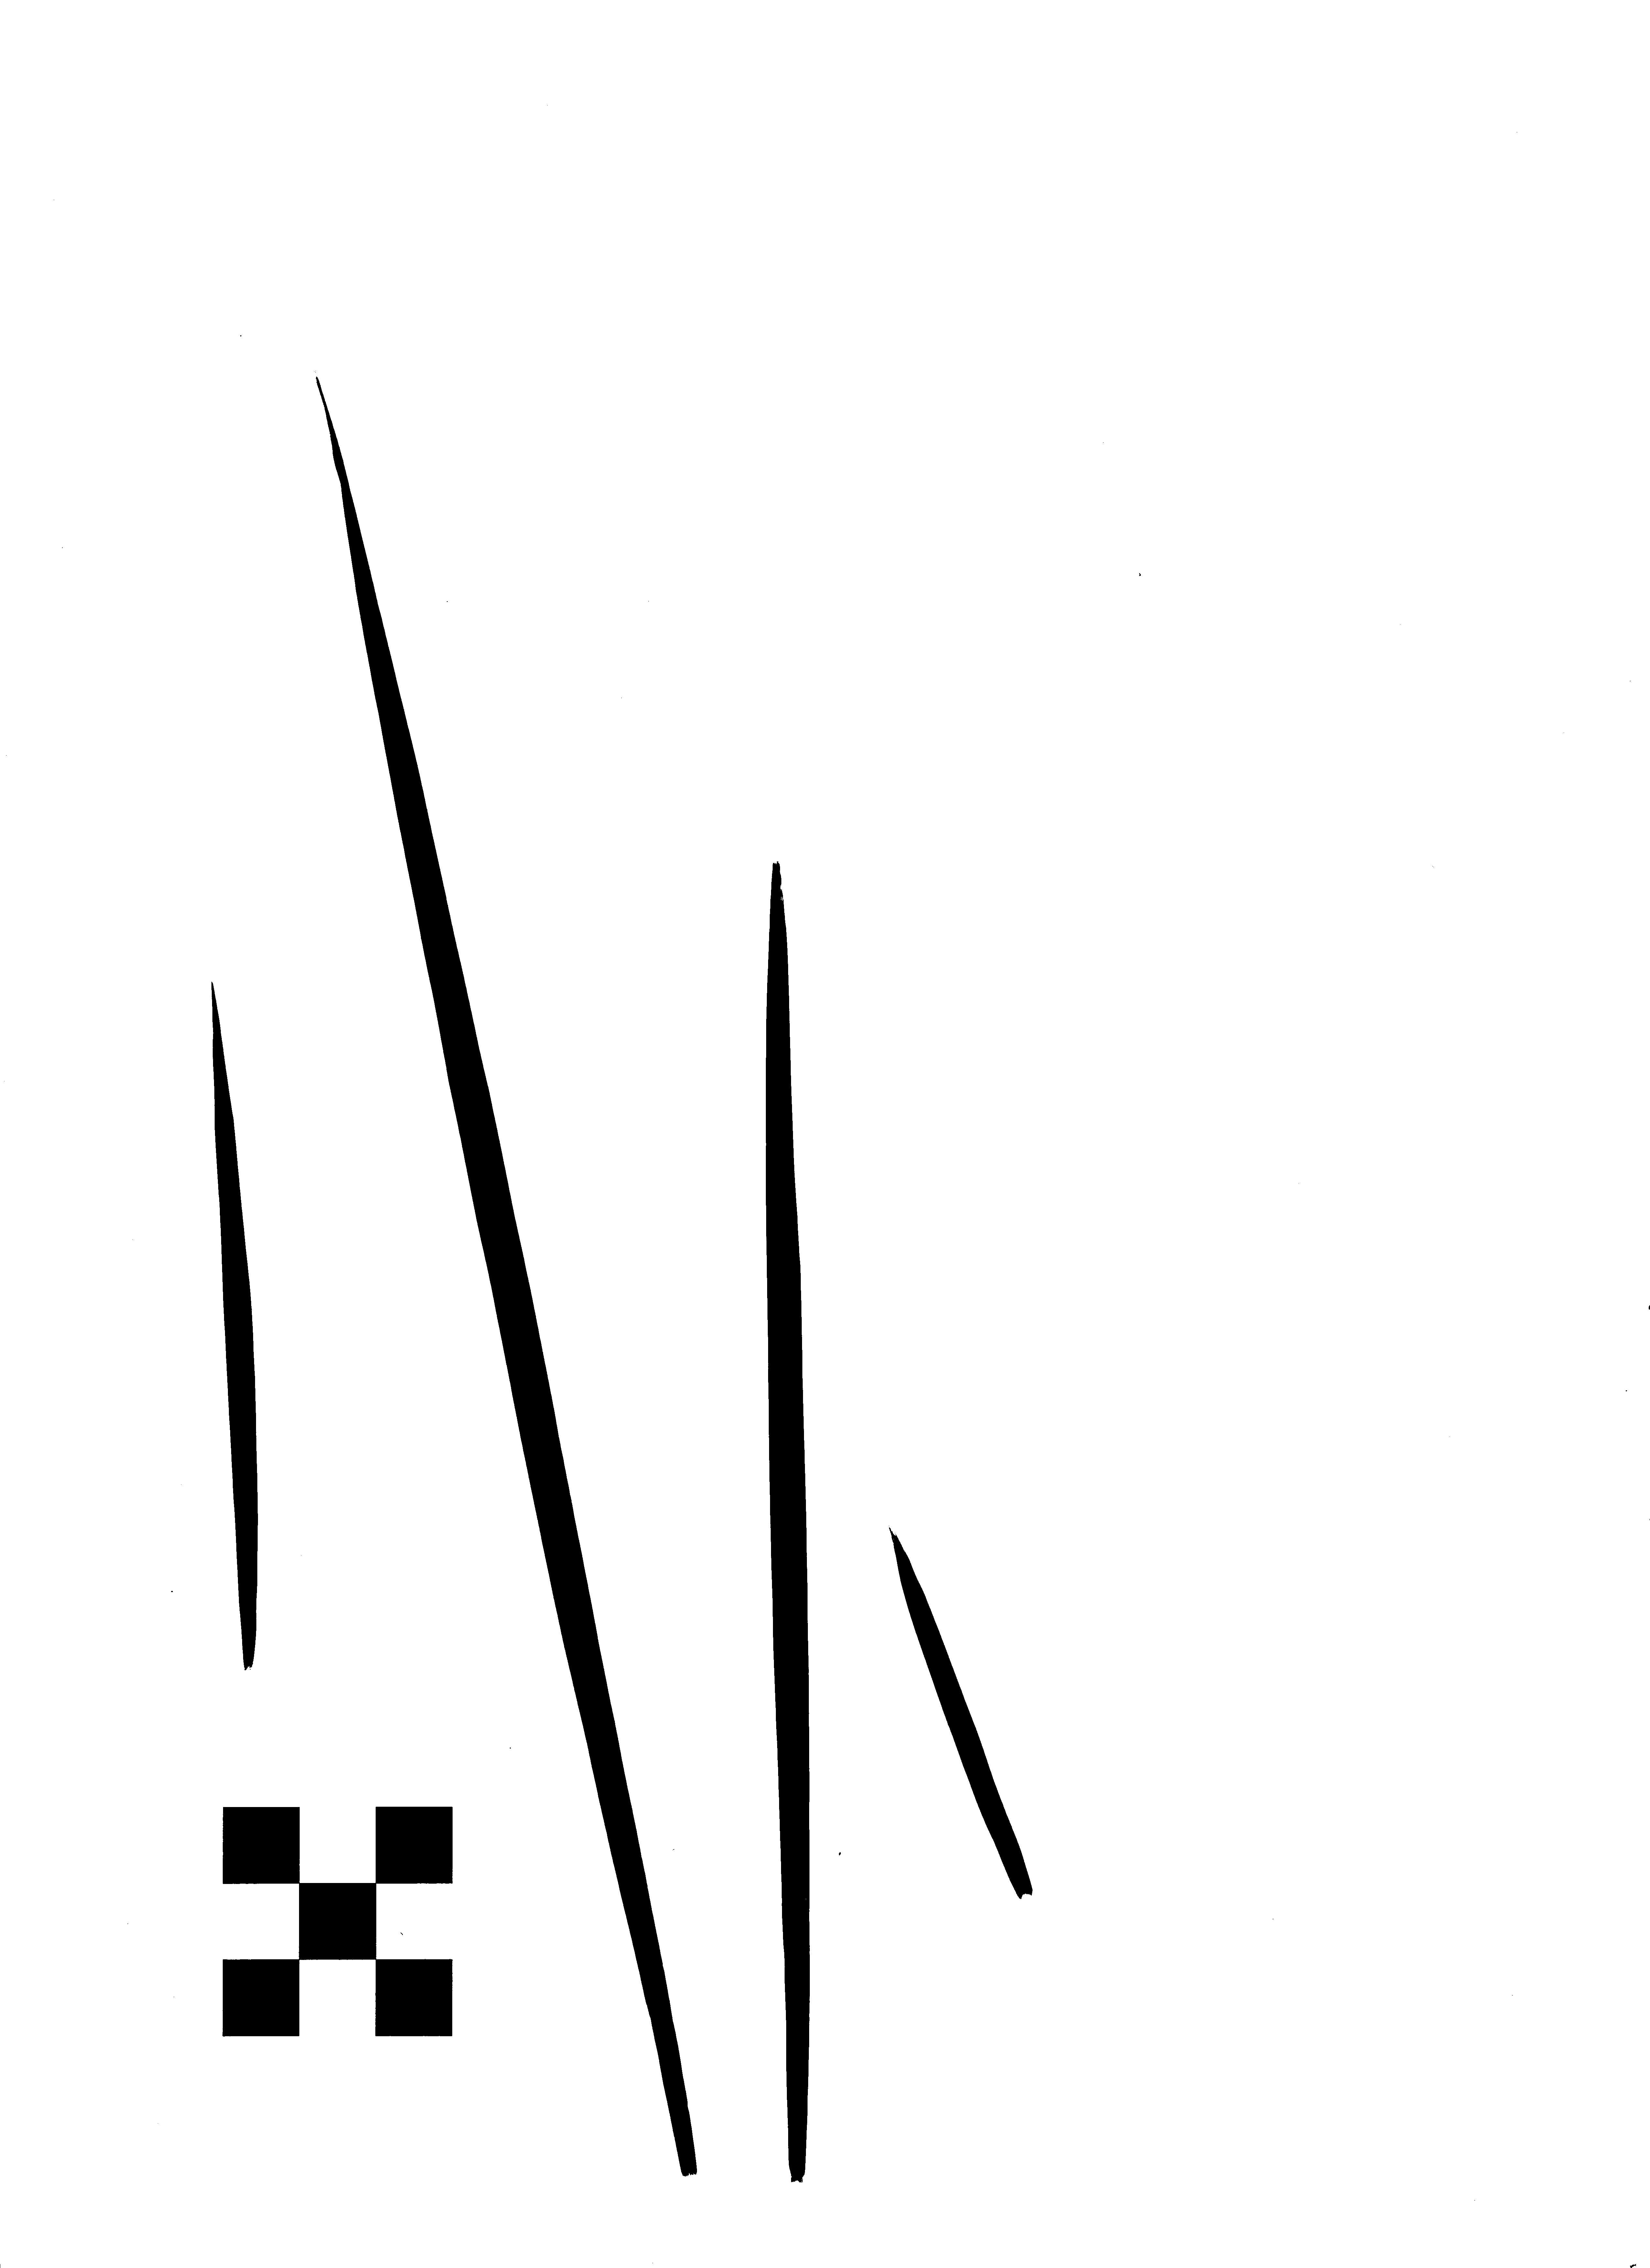
\includegraphics[width=.8\textwidth, frame]{chap2/Cch_moli_A_1to4_mod}
		\caption{image binarisée}
	\end{subfigure}
%    \caption{Caption place holder}
\caption{Scanne des feuilles}
\label{fig:scan_mol}
\end{figure}


\begin{figure}
	\centering
	\begin{subfigure}[t]{0.5\textwidth}
		\centering
		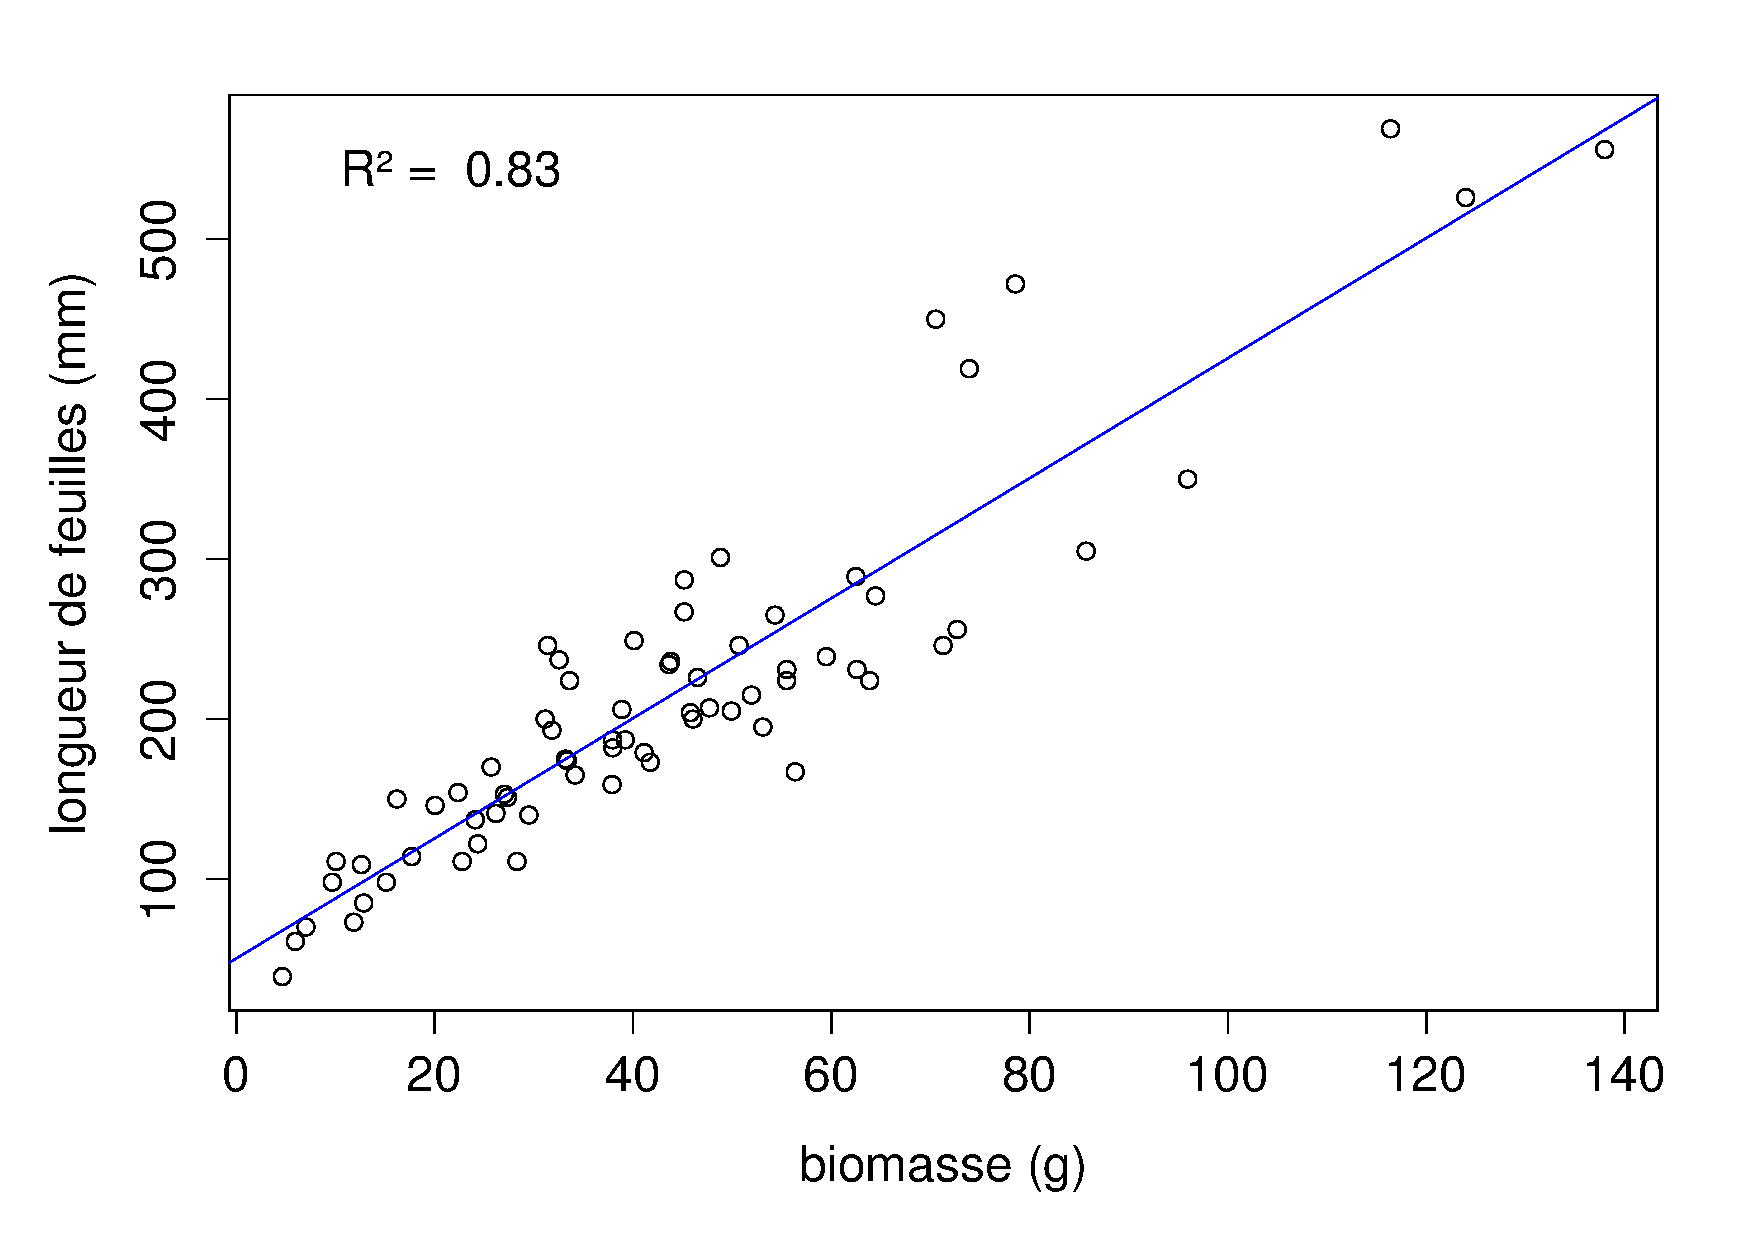
\includegraphics[width=\textwidth]{chap2/mol_lon_bioM}
		\caption{Molinia caerulea -- biomasse}
	\end{subfigure}%
	\begin{subfigure}[t]{0.5\textwidth}
		\centering
		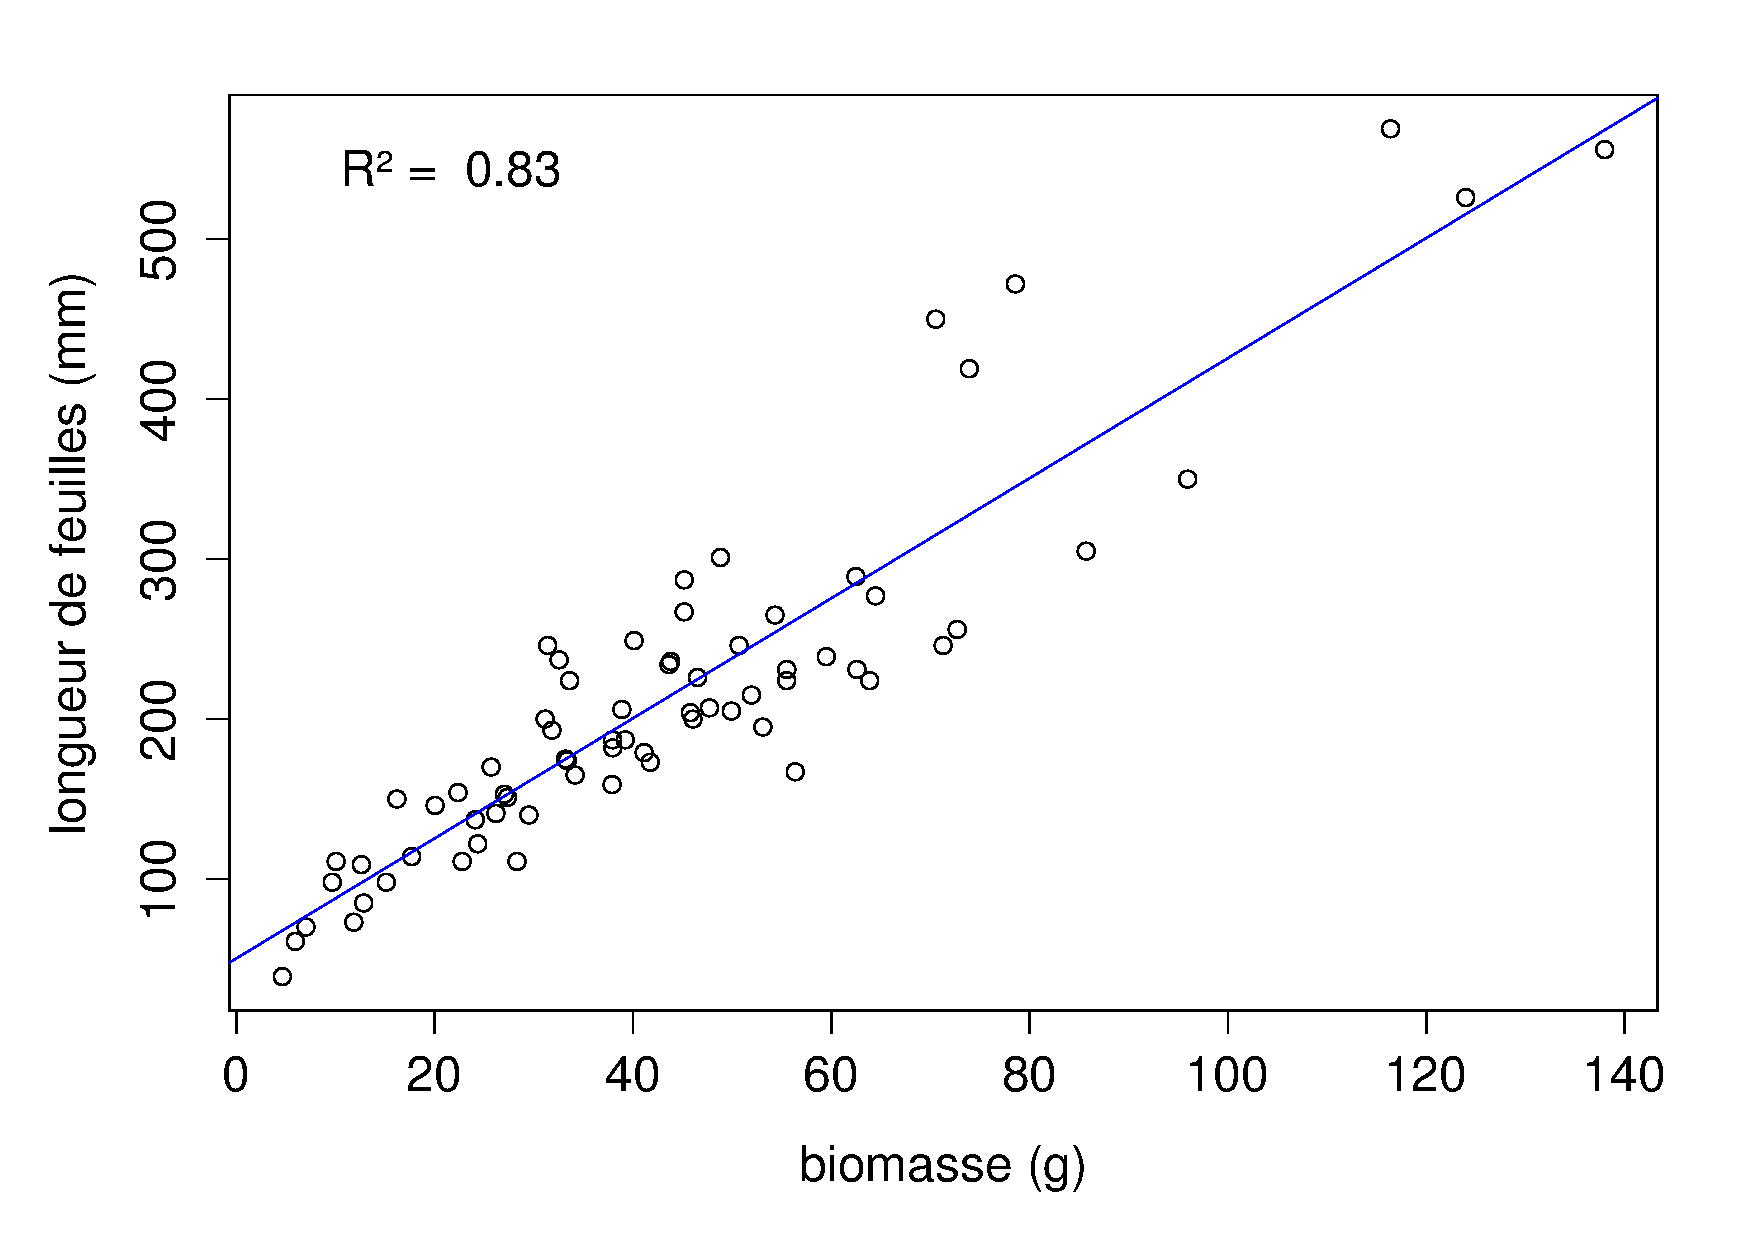
\includegraphics[width=\textwidth]{chap2/mol_lon_bioM}
		\caption{Eriophorum -- biomasse}
	\end{subfigure}
	
	
	\begin{subfigure}[t]{0.5\textwidth}
		\centering
		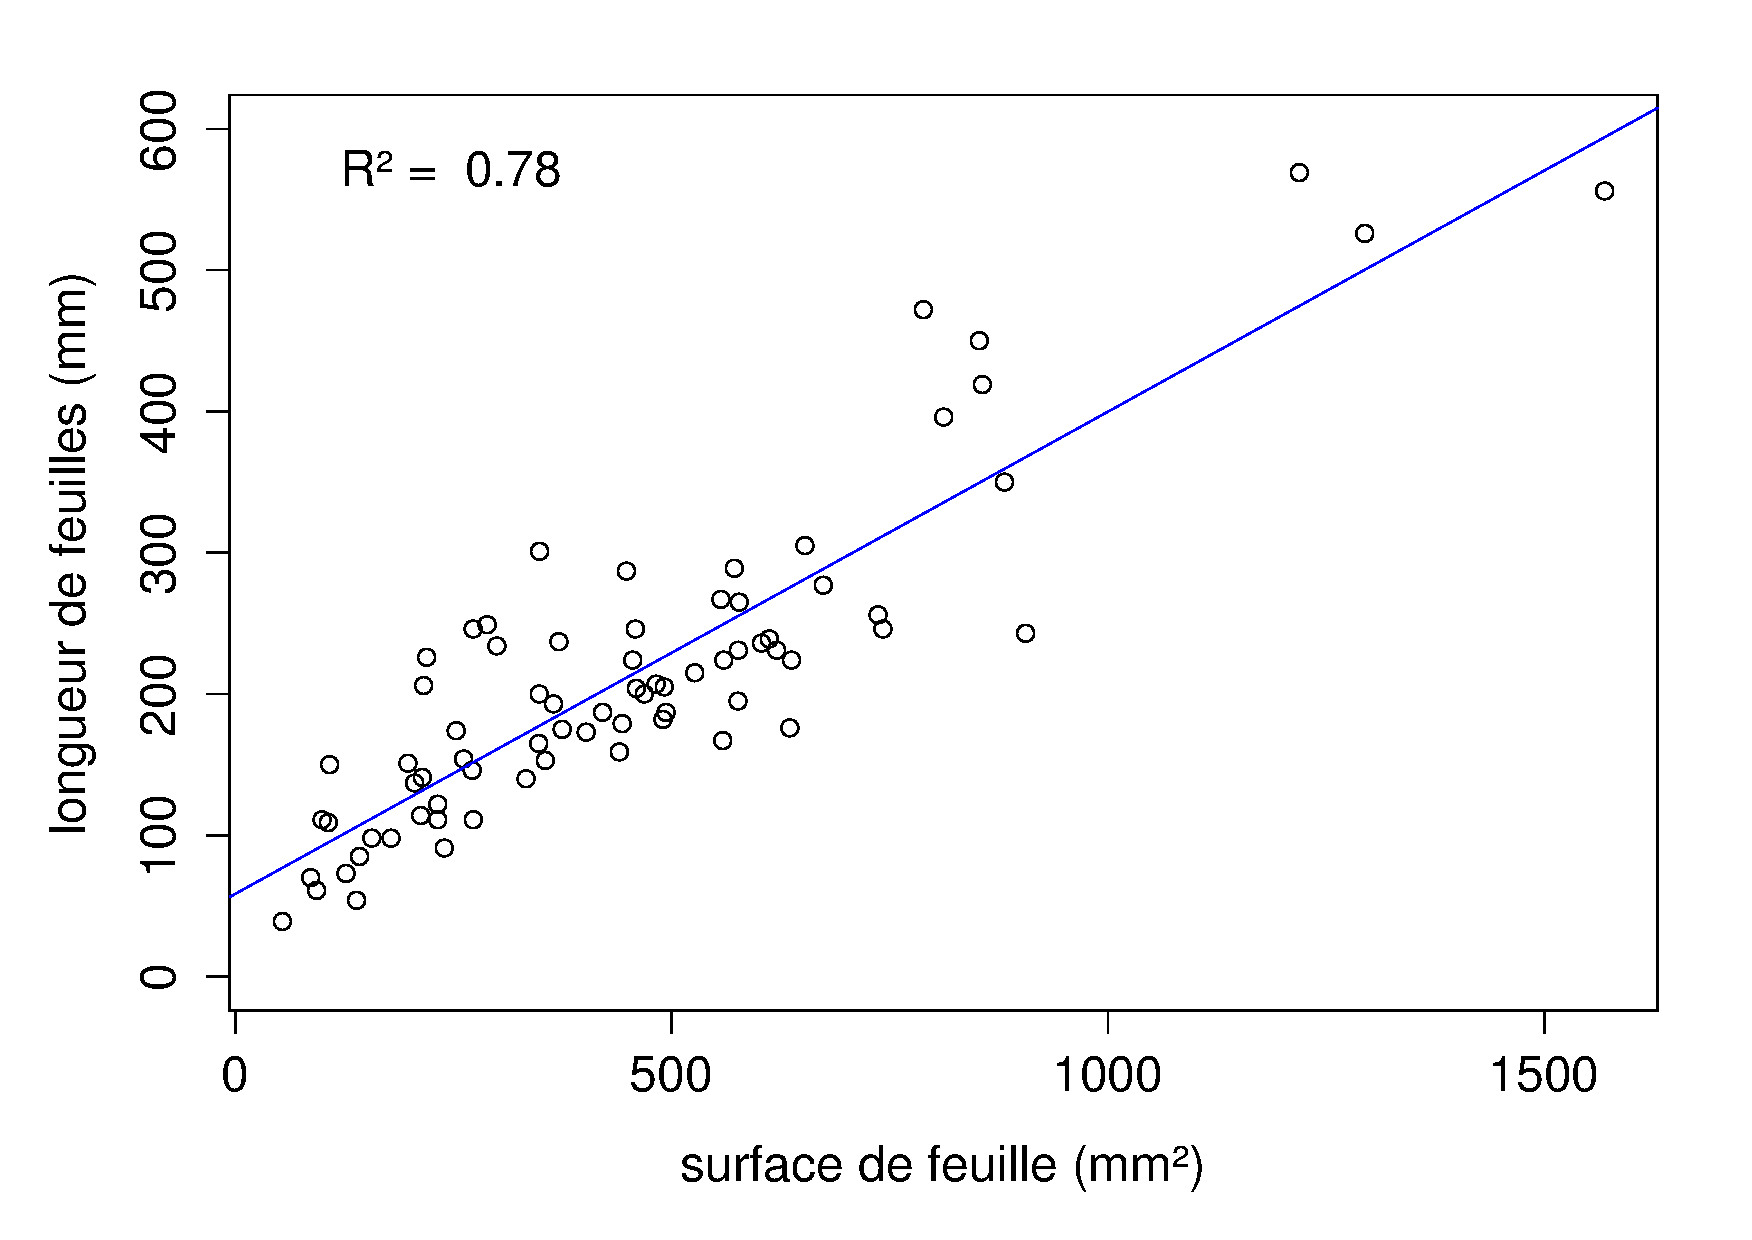
\includegraphics[width=\textwidth]{chap2/mol_lon_surf}
		\caption{Molinia caerulea -- surface}
	\end{subfigure}%
	\begin{subfigure}[t]{0.5\textwidth}
		\centering
		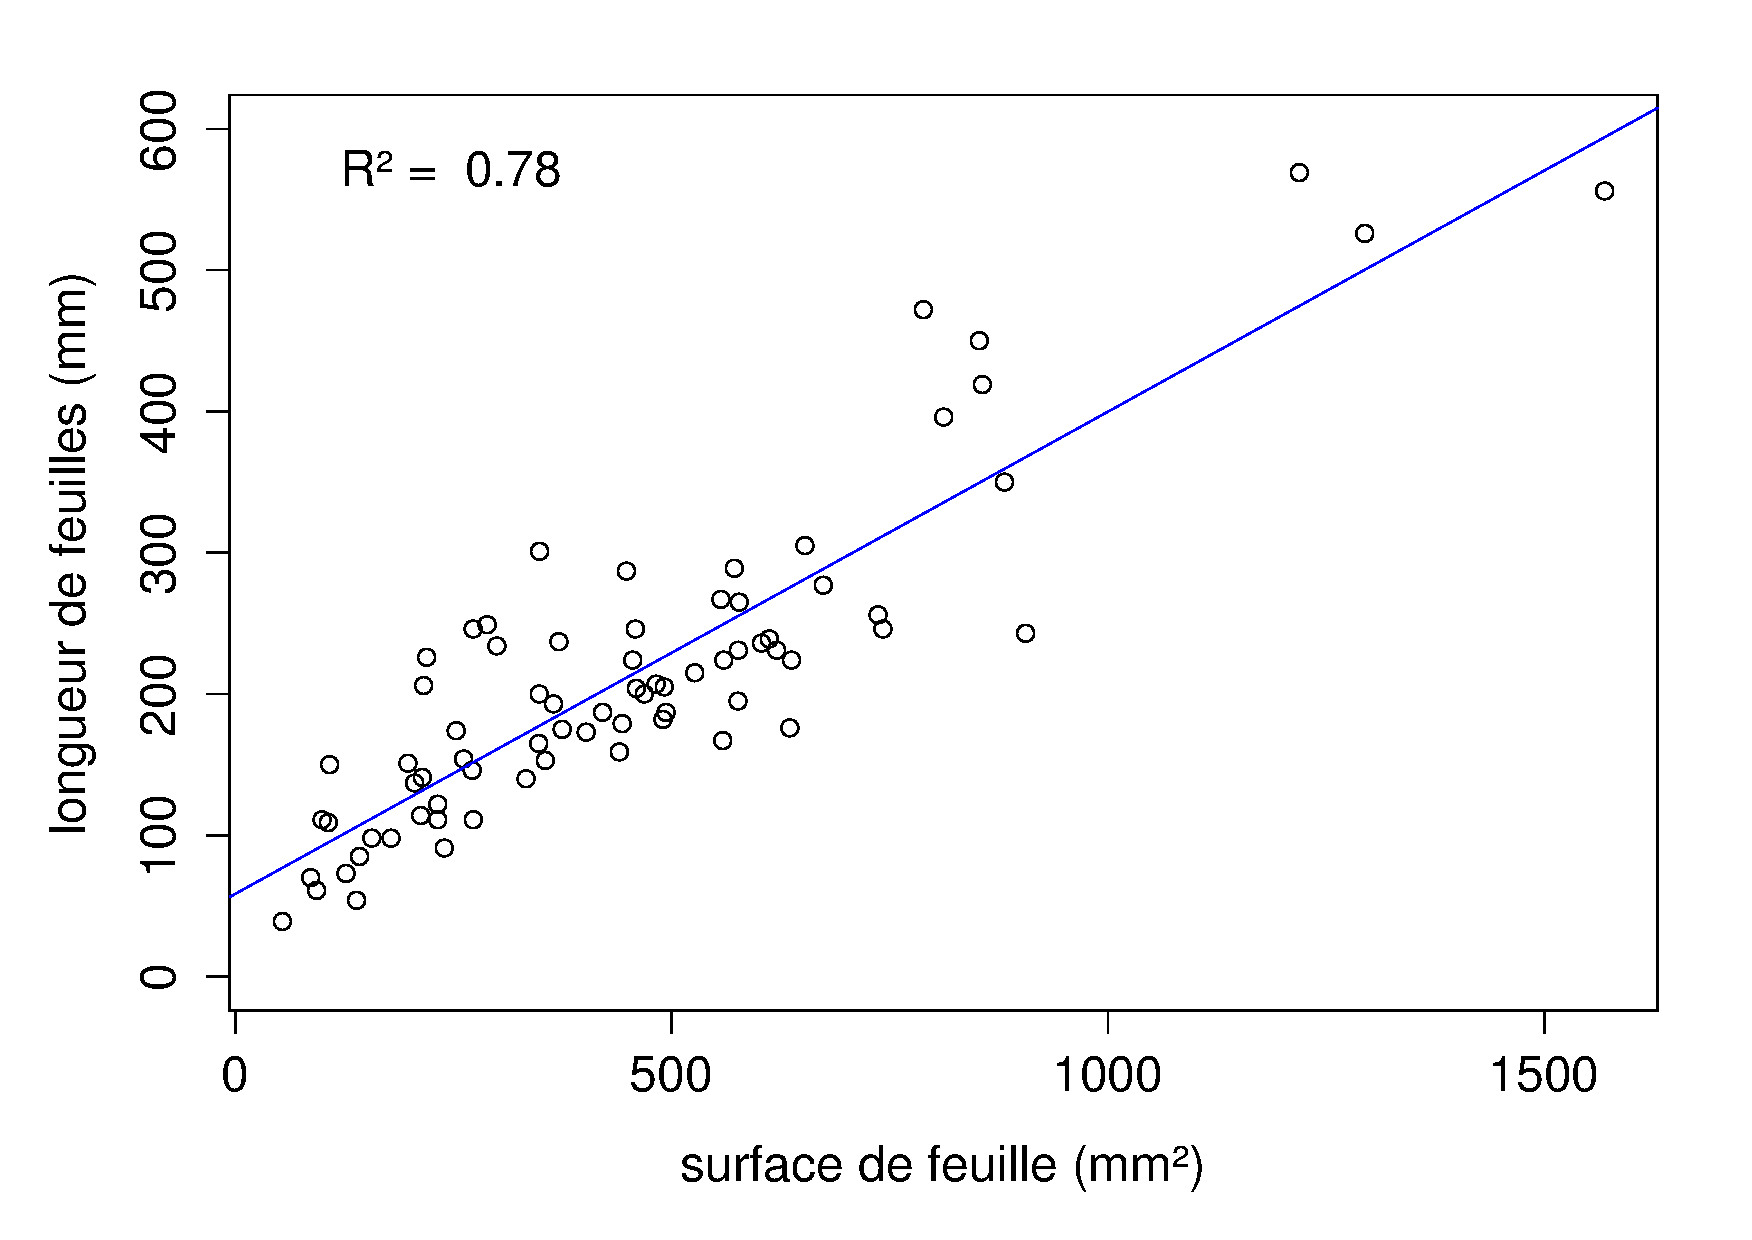
\includegraphics[width=\textwidth]{chap2/mol_lon_surf}
		\caption{Eriphorum -- surface}
	\end{subfigure}
%    \caption{Caption place holder}
\caption{Calibration de la biomasse herbacées pour \textit{molinia Caerulea} (a), pour \textit{eriophorum} (b) et de la surface de feuille pour \textit{molinia Caerulea} (c), pour \textit{eriophorum} (d) en fonction de la hauteur}
\label{fig:cal_herb}
\end{figure}


%\begin{figure}
%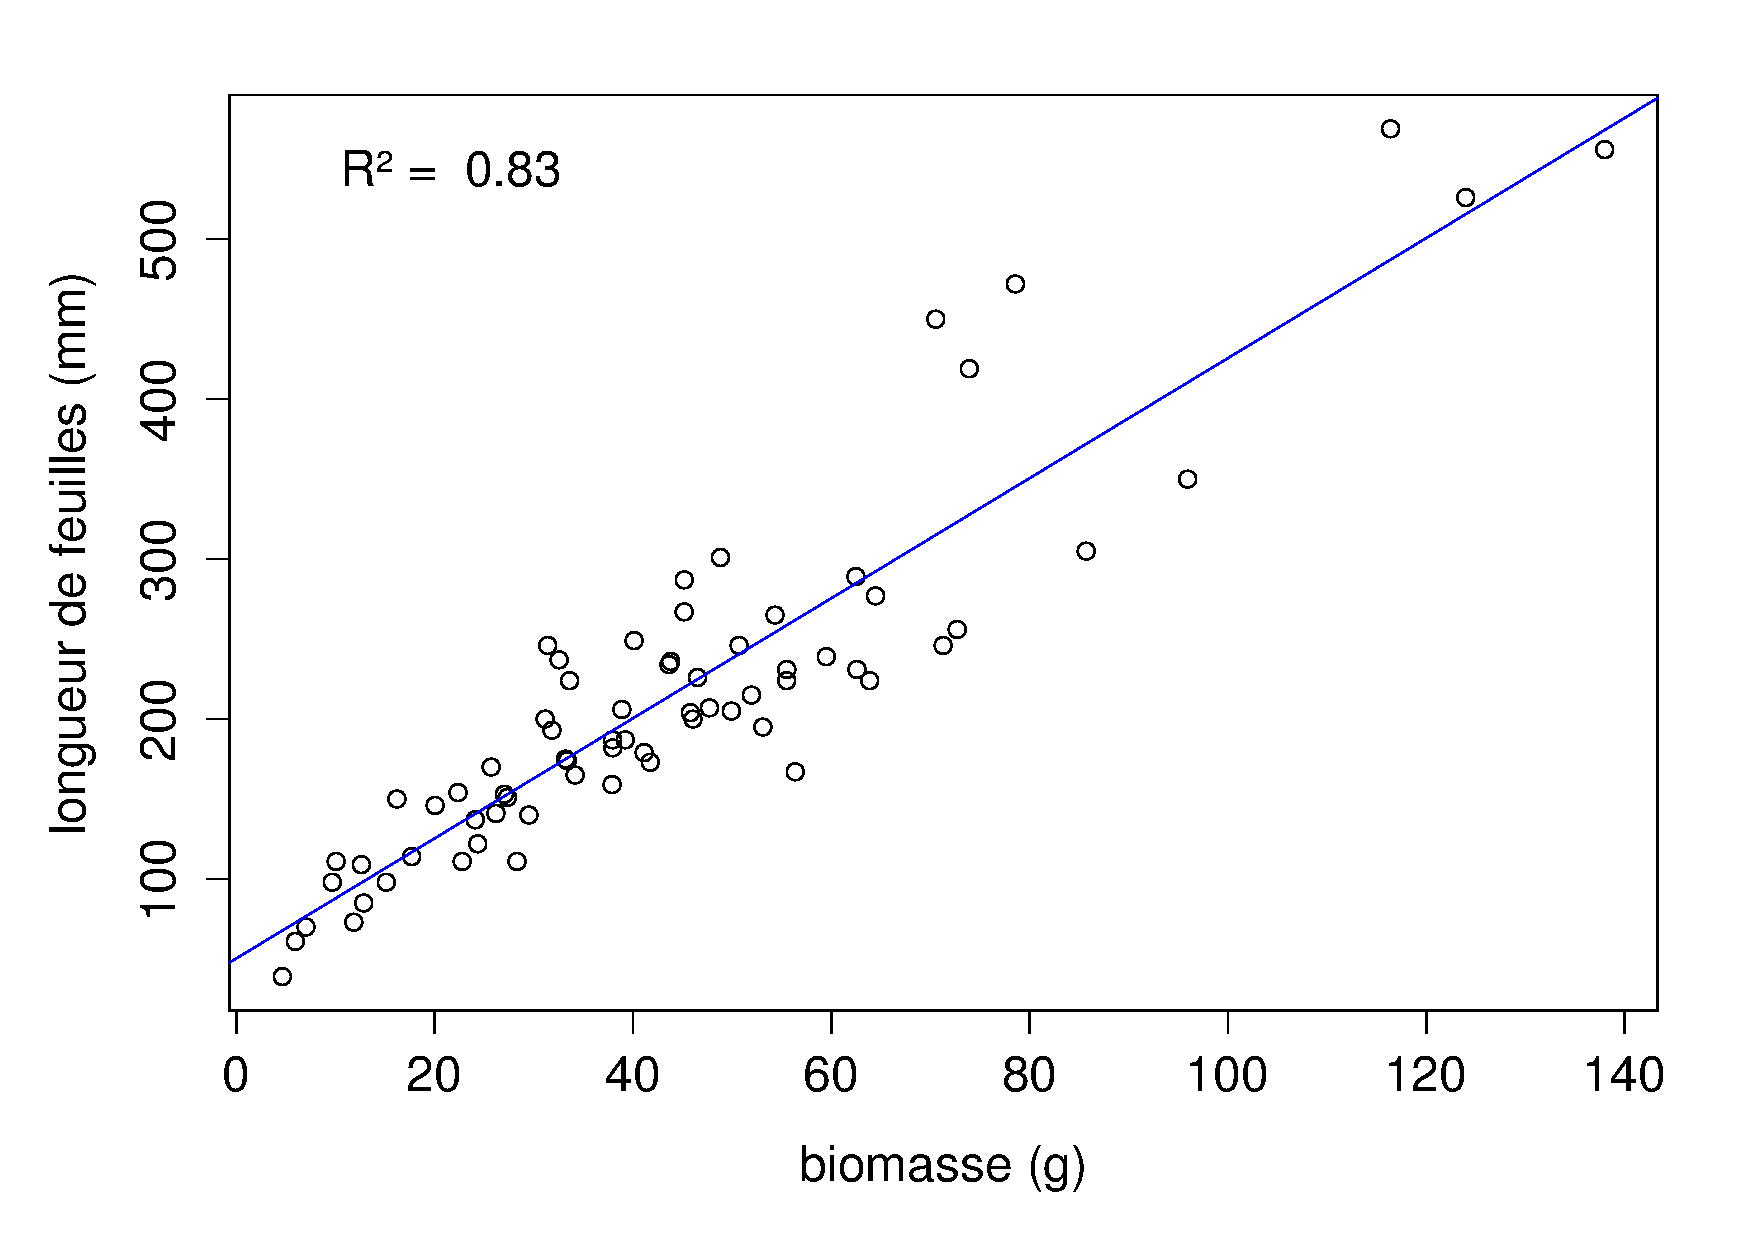
\includegraphics[width=.5\textwidth]{chap2/mol_lon_bioM}
%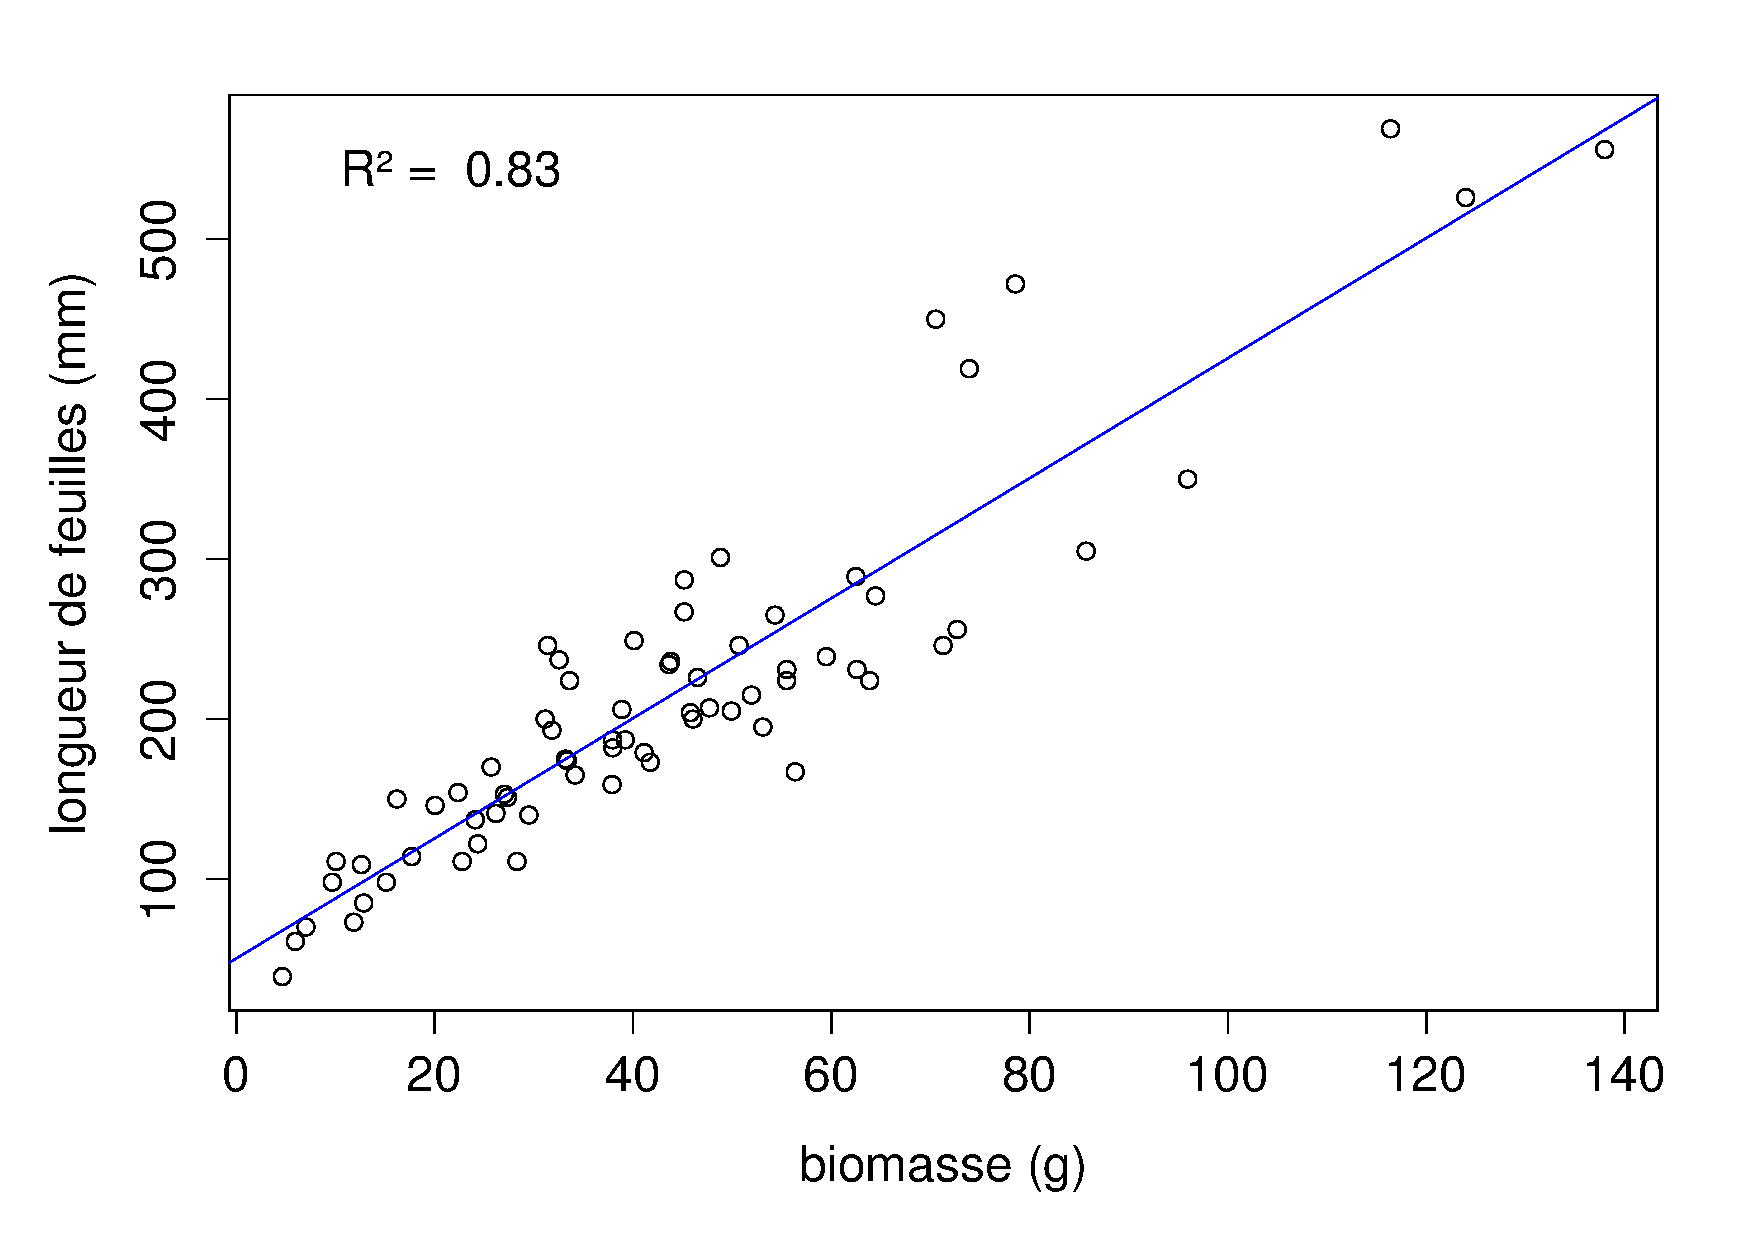
\includegraphics[width=.5\textwidth]{chap2/mol_lon_bioM}
%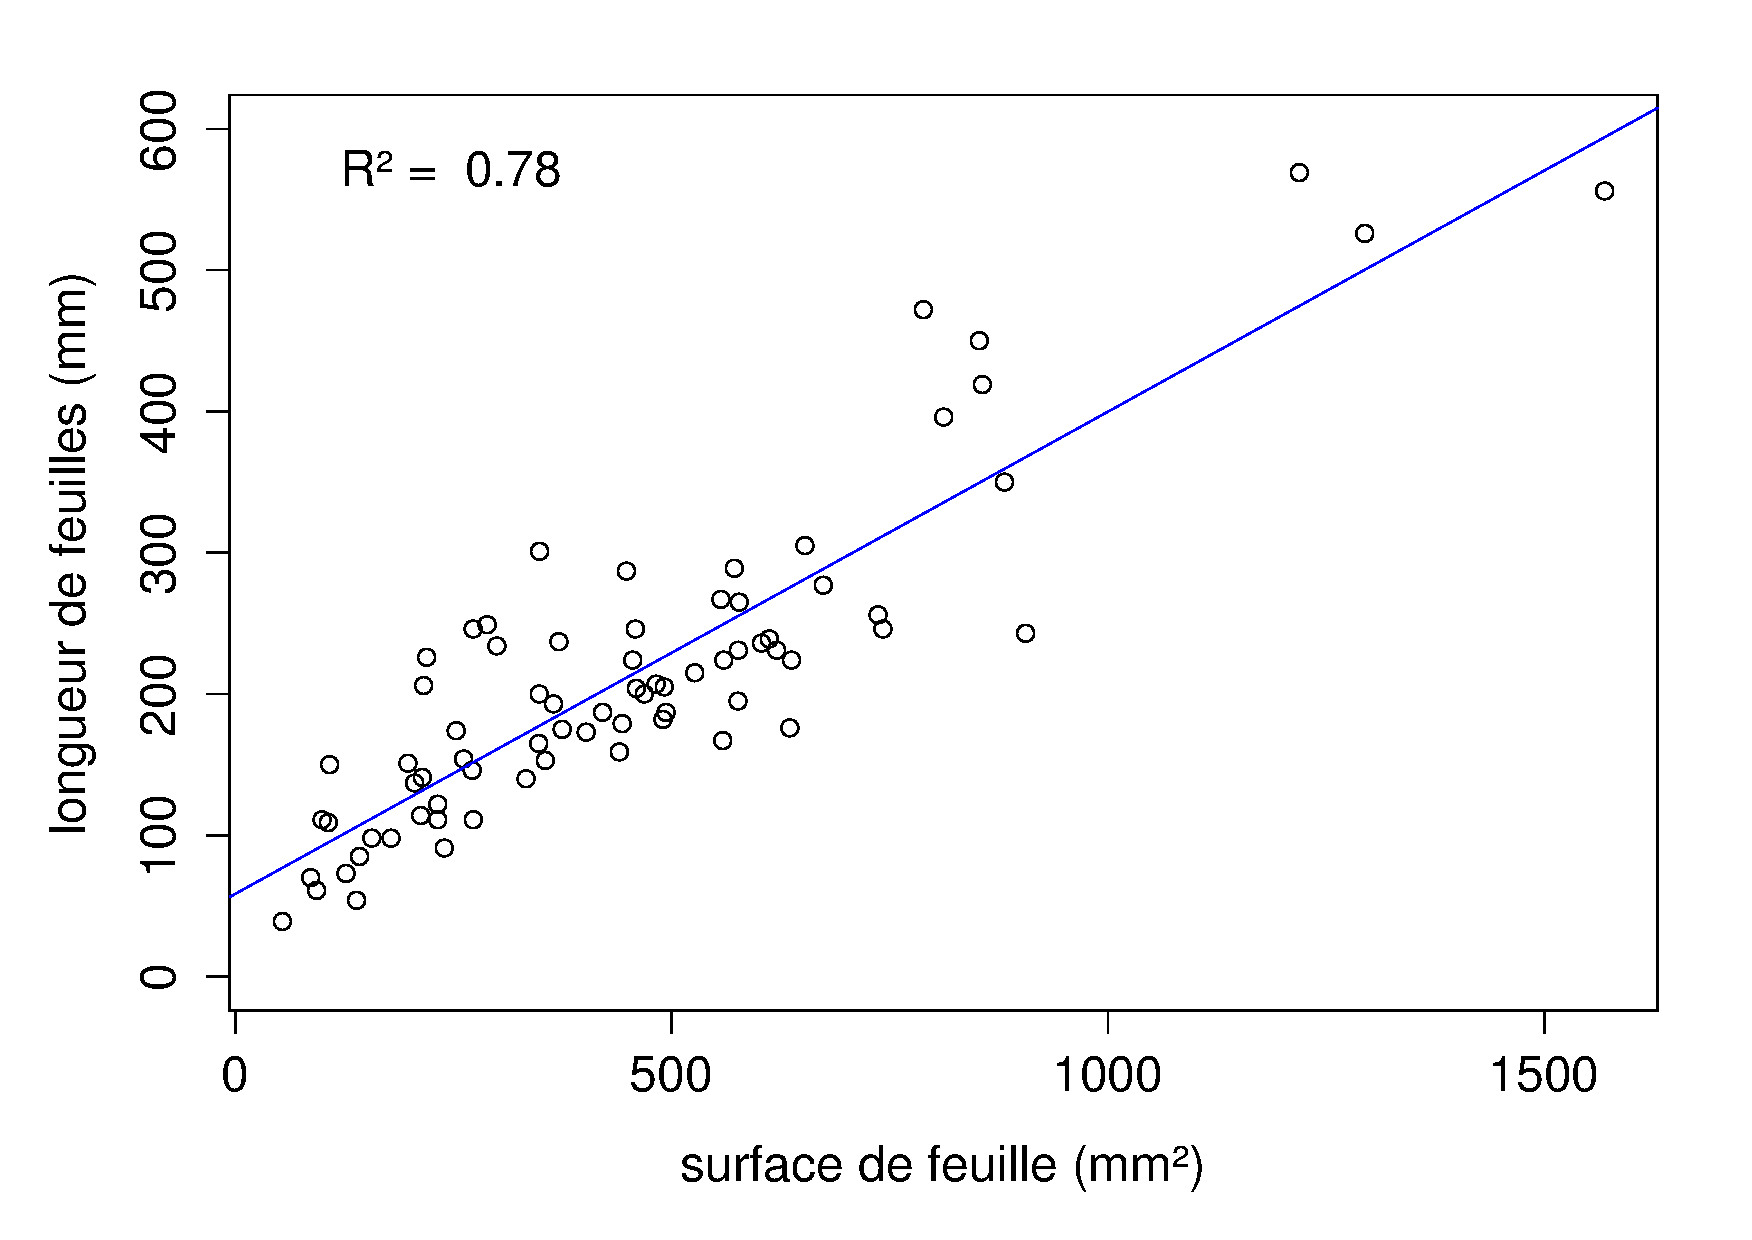
\includegraphics[width=.5\textwidth]{chap2/mol_lon_surf}
%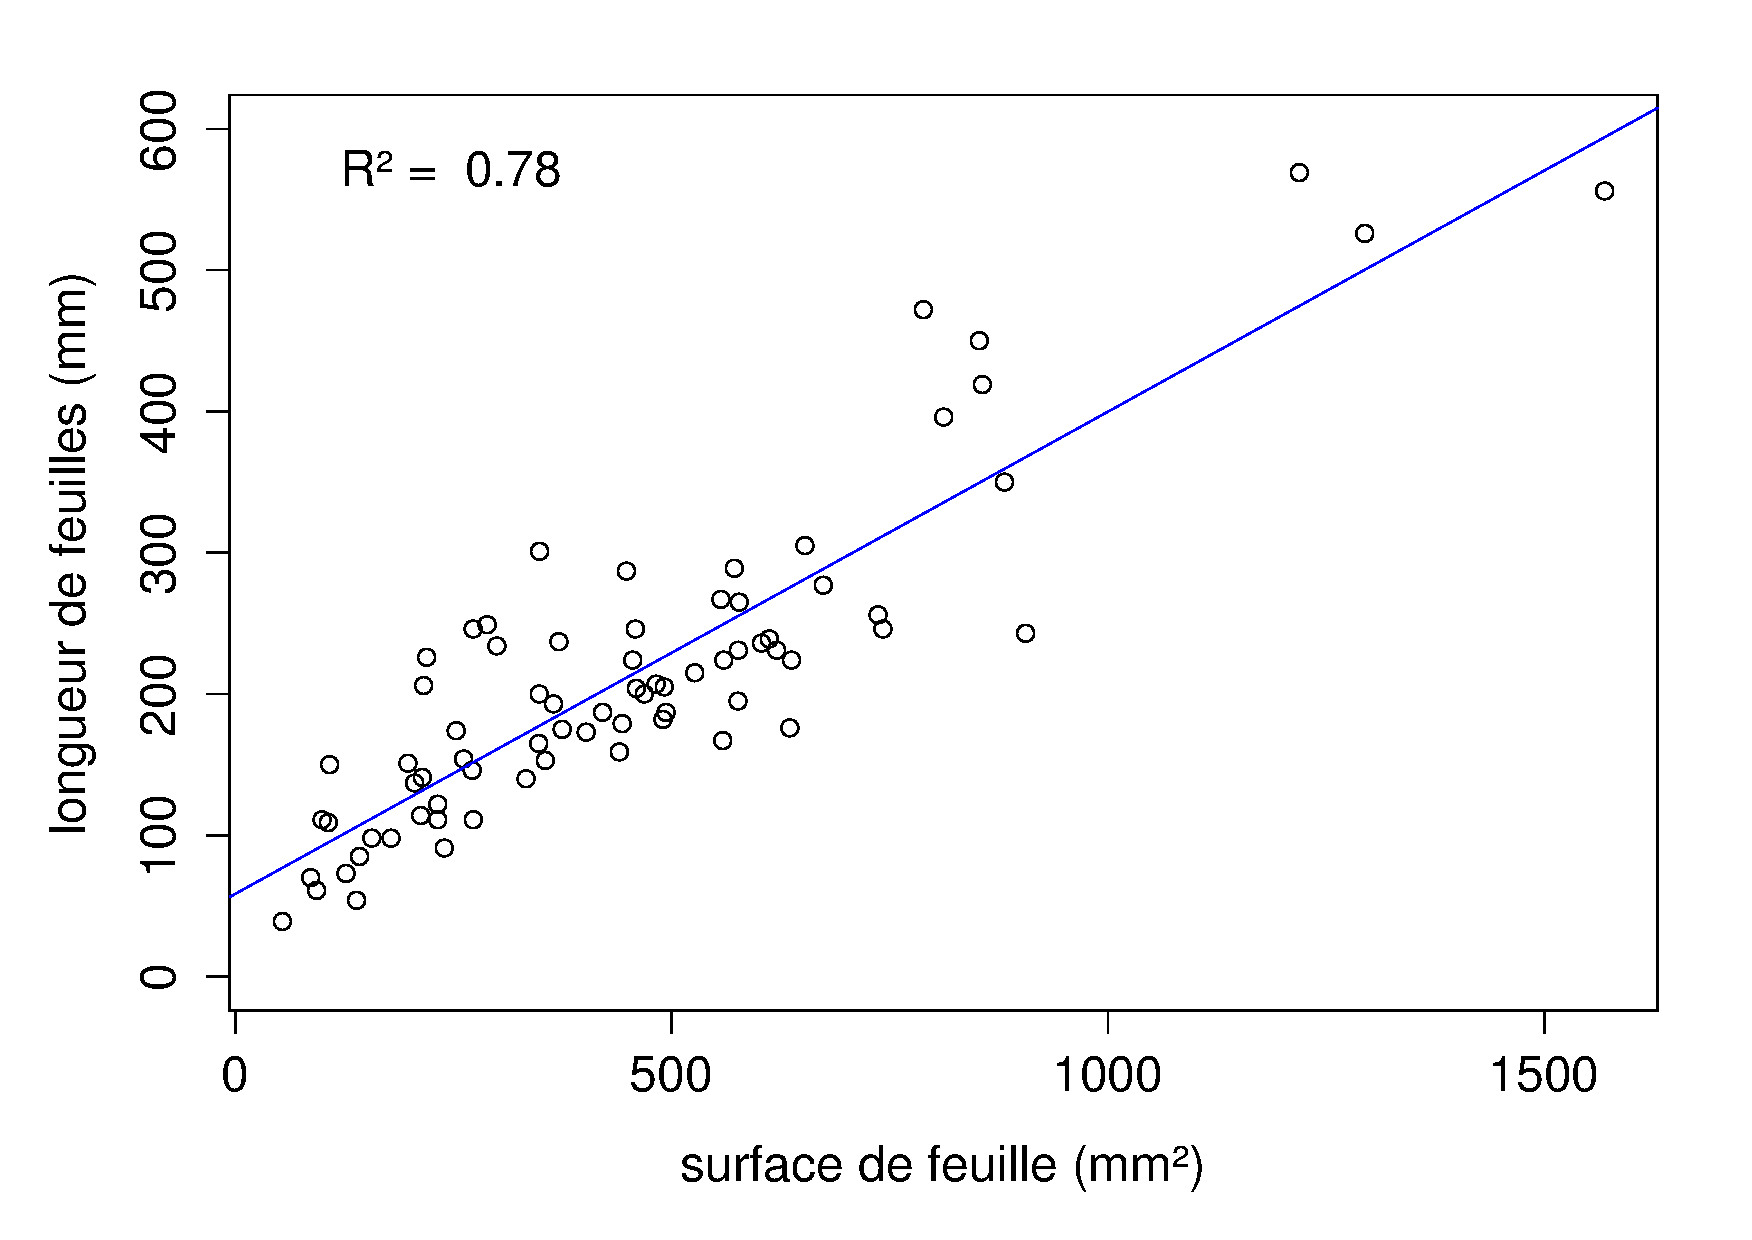
\includegraphics[width=.5\textwidth]{chap2/mol_lon_surf}
%\caption{Calibration de la biomasse herbacées pour \textit{molinia Caerulea} (a), pour \textit{eriophorum} (b) et de la surface de feuille pour \textit{molinia Caerulea} (c), pour \textit{eriophorum} (d) en fonction de la hauteur}
%\label{fig:cal_herb}
%\end{figure}